\section{Compacidad y conexión}


\begin{ejercicio}
Probar que dos normas definidas en un mismo espacio vectorial, que dan lugar a los mismos conjuntos acotados, han de ser equivalentes.\\

\noindent
Ya vimos en teoría que dos normas equivalentes en un mismo espacio vectorial dan lugar a los mismos conjuntos acotados, y aquí se nos pide probar el recíproco por lo que, una vez probado, que dos normas sean equivalentes es tanto como decir que dan lugar a los mismos conjuntos acotados.\\

\noindent
Sean pues $\|\cdot\|_1, \|\cdot\|_2$ dos normas definidas en $X$ que dan lugar a los mismos conjuntos acotados, probemos que $\exists \lm,\rho \in \mathbb{R}^+$ de forma que:
\begin{equation*}
    \lm \|x\|_1 \leq \|x\|_2 \leq \rho \|x\|_1 \qquad \forall x\in X
\end{equation*}
Para ello, consideramos $B_1 = \{x\in X : \|x\|_1 \leq 1\}$, que obviamente es un conjunto acotado para $\|\cdot\|_1$, luego también para $\|\cdot\|_2$, es decir, podemos encontrar $C\in \mathbb{R}^+$ de forma que $\|x\|_2 \leq C$ $\forall x\in B_1$. Como podemos escrbir:
\begin{equation*}
    x = \|x\|_1 \dfrac{x}{\|x\|_1} \qquad \forall x\in X
\end{equation*}
Tenemos entonces que:
\begin{equation*}
    \|x\|_2 = \|x\|_1 \left\|\dfrac{x}{\|x\|_1}\right\|_2 \stackrel{(\ast)}{\leq} C\|x\|_1 \qquad \forall x\in X
\end{equation*}
Donde en $(\ast)$ hemos usado que $\nicefrac{x}{\|x\|_1} \in B_1$ para todo $x\in X$, por lo que $\|\nicefrac{x}{\|x\|_1}\|_2 \leq C$. Aprovechando la simetría de la situación, podemos repetir este mismo razonamiento para $B_2 = \{x\in X : \|x\|_2 \leq 1\}$, obteniendo $C'\in \mathbb{R}^+$ de forma que:
\begin{equation*}
    \|x\|_1 \leq C' \|x\|_2 \qquad \forall x\in X
\end{equation*}
En definitiva, tenemos que:
\begin{equation*}
    \dfrac{1}{C'}\|x\|_1 \leq \|x\|_2 \leq C\|x\|_1 \qquad \forall x\in X
\end{equation*}
Con $\nicefrac{1}{C'},C\in \mathbb{R}^+$, por lo que $\|\cdot\|_1$ y $\|\cdot\|_2$ son equivalentes.
\end{ejercicio}

\begin{ejercicio}
Dado un subconjunto \( A \) de un espacio normado, probar que las siguientes afirmaciones son equivalentes:
    \begin{enumerate}
        \item \( A \) está acotado.
        \item Si \( \{a_n\} \) es una sucesión de puntos de \( A \) y \( \{\lambda_n\} \) una sucesión de números reales tal que \( \{\lambda_n\} \rightarrow 0 \), entonces \( \{\lambda_n  a_n\} \rightarrow 0 \).
        \item Para toda sucesión \( \{a_n\} \) de puntos de \( A \) se tiene que \( \left\{\dfrac{a_n}{n}\right\} \rightarrow 0 \).
    \end{enumerate}
    ¿Significa esto que si \( \left\{\dfrac{a_n}{n}\right\} \rightarrow 0 \), entonces la sucesión \( \{a_n\} \) está acotada?\\

    \noindent
    Sea $(X,\|\cdot\|)$ el espacio normado sobre el que trabajemos, $A\subset X$, para este ejercicio usaremos la siguiente definición de convergencia de una sucesión de puntos de $A$: Si $\{a_n\}$ es una sucesión de puntos de $A$, decimos que converge a $a\in X$ si:
    \begin{equation*}
        \forall \varepsilon >0~\exists m\in \mathbb{N} : \|a_n - a\| < \varepsilon~\forall n\geq m
    \end{equation*}
    \begin{description}
        \item [$i)\Longrightarrow ii)$] Si $A$ está acotado, $\exists M\in \mathbb{R}^+$ de forma que $\|a\| \leq M$ para todo $a\in M$. En particular, $\|a_n\| \leq M$ para todo $n\in \mathbb{N}$. Dado $\varepsilon>0$, la convergencia de $\{\lm_n\}$ a 0 nos permite encontrar para $\nicefrac{\varepsilon}{M}$ un $m\in \mathbb{N}$ de forma que:
            \begin{equation*}
                |\lm_n| < \dfrac{\varepsilon}{M} \qquad \forall n\geq m
            \end{equation*}
            En definitiva:
            \begin{equation*}
                \|\lm_n a_n\| = |\lm_n| \|a_n\| < \dfrac{\varepsilon}{M} M = \varepsilon \qquad \forall n\geq m
            \end{equation*}
            Es decir, $\{\lm_n a_n\}\rightarrow 0$.
        \item [$ii)\Longrightarrow iii)$] En particular, $\{\frac{1}{n}\}$ es una sucesión de números reales convergente a 0.
        \item [$iii)\Longrightarrow i)$] Por reducción al absurdo, si suponemos que $A$ no está acotado, para cada $n\in \mathbb{N}$ podemos encontrar $a_n \in A$ con $\|a_n\| > n$. De esta forma, $\{a_n\}$ es una sucesión de puntos de $A$, por lo que $iii)$ nos dice que $\{\nicefrac{a_n}{n}\}\rightarrow 0$. Sin embargo:
            \begin{equation*}
                \left\|\dfrac{a_n}{n}\right\| = \dfrac{1}{n} \|a_n\| > \dfrac{n}{n} = 1 \qquad \forall n\in \mathbb{N}
            \end{equation*}
            Contradicción con que $\{\nicefrac{a_n}{n}\}\rightarrow 0$.
    \end{description}
    Esto no significa que si tengamos una sucesión $\{a_n\}$ de forma que $\{\frac{a_n}{n}\}\rightarrow 0$, entonces $\{a_n\}$ esté acotada, ya que si tomamos $a_n = \sqrt{n}$ para todo $n\in \mathbb{N}$, tenemos que:
    \begin{equation*}
        \left\{\dfrac{a_n}{n}\right\} = \left\{\dfrac{\sqrt{n}}{n}\right\} = \left\{\dfrac{1}{\sqrt{n}}\right\} \rightarrow 0
    \end{equation*}
    Pero sin embargo $\{a_n\} = \{\sqrt{n}\}$ no está acotada; de hecho, diverge.
\end{ejercicio}

\begin{ejercicio}
Probar que todo espacio métrico finito es compacto. Probar también que, en un conjunto no vacío \( E \) con la distancia discreta, todo subconjunto compacto de \( E \) es finito.\\

\noindent
Sea $(E,d)$ un espacio métrico finito y $\{x_n\}$ una sucesión de puntos de $E$, por ser $E$ finito ha de existir un elemento que se repita una cantidad infinita de veces, es decir, $\exists \alpha\in E$ de forma que $\forall n\in E$ $\exists m>n$ con $x_m = \alpha$. De esta forma, podemos construir una parcial $\{x_{\sigma(n)}\}$ que sea constantemente igual a $\alpha$, luego convergente; por lo que $E$ es compacto.\\

\noindent
Que una sucesión $\{x_n\}$ de puntos de $E\neq \emptyset $ sea convergente con la distancia discreta significa que $\exists x\in E$ tal que:
\begin{equation*}
    \forall \varepsilon>0~\exists m\in \mathbb{N} : d_{\text{disc}}(x_n,x) < \varepsilon~\forall n\geq m
\end{equation*}
En particular, como:
\begin{equation*}
    d_{\text{disc}}(x_n, x) = \left\{\begin{array}{ll}
            0 & \text{si y solo si\ } x_n = x \\
            1 & \text{si y solo si\ } x_n \neq x 
    \end{array}\right. \qquad \forall n\in \mathbb{N}
\end{equation*}
Para que $\{x_n\}$ sea convergente, como ha de cumplir la condición anterior para cada $\varepsilon >0$ (en particular, para $1>\varepsilon>0$), es necesario que exista un término a partir del cual todos los términos de $\{x_n\}$ sean iguales.\\

\noindent
Una vez discutida la convergencia en dicho espacio métrico, sea $A\subset E$ un conjunto copacto para la distancia discreta, supongamos que $A$ es infinito, por lo que podemos construir una sucesión $\{a_n\}$ con todos sus elementos distintos. Por ser $A$ compacto, existe una parcial $\{a_{\sigma(n)}\}$ convergente, es decir, tiene un término a partir del cual todos sus términos son iguales, pero como los términos de $\{a_{\sigma(n)}\}$ son en particular términos de $\{a_n\}$, estos serán todos distintos entre sí. Hemos llegado a una \underline{contradicción}, que venía de suponer que $A$ era infinito, por lo que $A$ es finito.
\end{ejercicio}

\begin{ejercicio}
Sea \( \{x_n\} \) una sucesión convergente de puntos de un espacio métrico y \( x = \lim\limits_{n \to \infty} x_n \). Probar que el conjunto \( A = \{x_n : n \in \mathbb{N}\} \cup \{x\} \) es compacto.\\

\noindent
Sea $\{a_n\}$ una sucesión de puntos de $A$:
\begin{itemize}
    \item Si $x$ aparece infinitas veces en $\{a_n\}$, podemos quedarnos con el subconjunto de $\mathbb{N}$ de aquellos índices de la sucesión cuyos términos coinciden con $x$, con lo que obtenemos una parcial de $\{a_n\}$ constantemente igual a $x$, luego convergente. 
    \item De forma análoga, si existe un $j\in \mathbb{N}$ de forma que $a_j$ aparece infinitas veces en $\{a_n\}$, podemos obtener una parcial constantemente igual a $a_j$, luego convergente.
    \item En otro caso, construiremos una parcial de $\{a_n\}$ de forma recursiva, de forma que en dicha parcial no aparezca $x$:
        \begin{itemize}
            \item El primer término será el primer término de la sucesión $\{a_n\}$ que sea distinto de $x$, con lo que será de la forma $x_j$ para cierto $j\in \mathbb{N}$, que se alcanzará en alguna posición $k\in \mathbb{N}$: $a_k = x_j$. Definimos $\sigma(1) = k$.
            \item Conocido el último término de la parcial, $a_{\sigma(n)}$, que coincidirá con $x_m$ para cierto $m\in \mathbb{N}$, como el conjunto $\{x_n : n \leq m\}$ contiene $m$ elementos y no hay ningún elemento que se repita de forma infinita, podremos encontrar un elemento $a_k$ con $k > \sigma(n)$ de forma que $a_k = x_j$, para cierto $j>m$.

                En dicho caso, definimos $\sigma(n+1) = k$.
        \end{itemize}

        Lo que hemos hecho ha sido construir una parcial $\{a_{\sigma(n)}\}$ de elementos del conjunto $\{x_n : n\in \mathbb{N}\}$ de forma que si $n>m$, entonces el elemento $a_{\sigma(n)}$ de la sucesión $\{x_n\}$ aparece antes en dicha sucesión que el elemento $a_{\sigma(m)}$. En definitiva, resulta que $\{a_{\sigma(n)}\}$ también es una parcial de $\{x_n\}$, por lo que ha de ser convergente, y al mismo límite $x$.
\end{itemize}
En definitiva, cualquier sucesión de puntos de $A$ admite una parcial convergente, luego $A$ es compacto.
\end{ejercicio}

\begin{ejercicio}
Probar que, si \( E \) es un espacio métrico compacto, y \( A \) es un subconjunto infinito de \( E \), entonces \( A' \neq \emptyset \).\\

\noindent
Como $A$ es infinito, podemos tomar $\{a_n\}$, una sucesión de puntos de $A$ todos ellos distintos entre sí, es decir:
\begin{equation*}
    a_n = a_m \Longleftrightarrow n = m
\end{equation*}
En dicho caso, como $E$ es compacto, existe una parcial convergente a un punto de $E$: $\exists \{a_{\sigma(n)}\}\rightarrow x\in E$. Veamos que $x\in A'$, con lo que $A' \neq \emptyset $. Para ello, sea $U\in \cc{U}(x)$, como $\{a_{\sigma(n)}\} \rightarrow x$, sabemos que $\exists m\in \mathbb{N}$ de forma que:
\begin{equation*}
    x_n \in U \qquad \forall m\geq n
\end{equation*}
Por tanto, tendremos que $U\cap (A\setminus \{x\}) \neq \emptyset $, luego $x\in A'$.
\end{ejercicio}

\begin{ejercicio}
Sea \( E \) un espacio métrico con distancia \( d \) y \( K \) un subconjunto compacto de \( E \). Probar que, para cada \( x \in E \), existe un punto \( k_x \in K \) tal que \( d(x, k_x) \leq d(x, k) \) para todo \( k \in K \).\\

\noindent
Dado $x\in E$, definimos $f:K\rightarrow \mathbb{R}$ dada por:
\begin{equation*}
    f(k) = d(x,k) \qquad \forall k\in K
\end{equation*}
$f$ es continua, ya que:
\begin{equation*}
    |f(t) - f(s)| = |d(x,t) - d(x,s)| \leq d(t,s) \qquad \forall t,s\in K
\end{equation*}
Y como $K$ es compacto, tenemos que $f(K) = \{d(x,k) : k\in K\} \subseteq \mathbb{R}$ es compacto, luego existe su mínimo, es decir, $\exists k_x \in K$ de forma que:
\begin{equation*}
    d(x,k_x) \leq d(x,k) \qquad \forall k\in K
\end{equation*}
Como queríamos probar.
\end{ejercicio}

\begin{ejercicio}
Sea \( A \) un subconjunto cerrado de \( \mathbb{R}^N \) y consideremos en \( \mathbb{R}^N \) cualquier distancia \( d \) que genere la topología usual. Probar que, para todo \( x \in \mathbb{R}^N \), se puede encontrar un \( a_x \in A \), tal que \( d(x, a_x) \leq d(x, a) \) para todo \( a \in A \).\\

\noindent
Sea $x\in \mathbb{R}^N$, si $A = \emptyset $ el resultado es cierto. Si $A\neq \emptyset $, consideramos (existe por ser el de la derecha un conjunto no vacío y minorado por 0):
\begin{equation*}
    d(x,A) = \inf \{d(x,a):a\in A\}
\end{equation*}
Por la caracterización del ínfimo, sabemos que existe una sucesión de puntos del conjunto convergente a él, es decir, existe $\{a_n\}$ con $a_n \in A$ para todo $n\in \mathbb{N}$ de forma que $\{d(x,a_n)\} \rightarrow d(x,A)$. Hemos visto en teoría que toda sucesión convergente está acotada, luego $\{d(x,a_n)\}$ está acotada, es decir, $\exists R\in \mathbb{R}^+$ de forma que $d(x,a_n)\leq R$ $\forall n\in \mathbb{N}$, por lo que $a_n \in B(x,R+1)$ $\forall n\in \mathbb{N}$, de donde la sucesión $\{a_n\}$ está acotada. Por el Teorema de Bolzano-Weierstrass, admite una parcial convergente $\{a_{\sigma(n)}\} \rightarrow a_x \in \overline{A} = A$.

Si nos fijamos en el ejercicio anterior, no usamos que $K$ era compacto para probar que $f$ era continua, por lo que si volvemos a definir $f:A\rightarrow \mathbb{R}$ dada por:
\begin{equation*}
    f(a) = d(x,a) \qquad \forall a\in A
\end{equation*}
Tenemos que $f$ es continua, ya que:
\begin{equation*}
    |f(a) - f(b)| = |d(x,a) - d(x,b)| \leq d(a,b) \qquad \forall a,b\in A
\end{equation*}
Finalmente, de $\{a_{\sigma(n)}\} \rightarrow a_x$ y la continuidad de $f$, concluimos que:
\begin{equation*}
    \{d(x,a_{\sigma(n)})\} = \{f(a_{\sigma(n)})\} \rightarrow f(a_x) = d(x,a_x)
\end{equation*}
Sin embargo, $\{d(x,a_{\sigma(n)})\}$ es una parcial de $\{d(x,a_n)\}$, que era convergente a $d(x,A)$, por lo que $d(x,a_x) = d(x,A)$. En definitiva, tenemos que:
\begin{equation*}
    d(x,a_x) = d(x,A) \leq d(x,a) \qquad \forall a\in A
\end{equation*}
\end{ejercicio}

\begin{ejercicio}
Sea \( F \) un conjunto no vacío con la distancia discreta. Probar que si \( E \) es un espacio métrico conexo, toda función continua de \( E \) en \( F \) es constante.\\

\noindent
Es bien sabido ya que si $F$ es un conjunto no vacío con la distancia discreta, entonces esta distancia genera la topología discreta:
\begin{equation*}
    \cc{T}_{d_{\text{disc}}} = \cc{T}_{\text{disc}} = \cc{P}(F)
\end{equation*}
Demostraremos un sencillo Lema para probar este ejercicio:

\begin{lema*}
    Si $(X,\cc{T}_{\text{disc}})$ es un espacio topológico con la topología discreta y $A\subset X$ contiene al menos dos elementos distintos, entonces $A$ no es conexo.
    \begin{proof}
        Sean, pues $x,y\in A$ con $x\neq y$. En dicho caso, tomando:
        \begin{equation*}
            U = \{x\}, \qquad V = A\setminus \{x\}
        \end{equation*}
        Tenemos que $U,V \in \cc{P}(X) = \cc{T}_{\text{disc}}$, $U,V \neq \emptyset $, así como que:
        \begin{equation*}
            U\cap V = \{x\} \cap (A\setminus \{x\}) = \emptyset \qquad U\cup V = \{x\}\cup (A\setminus \{x\}) = A
        \end{equation*}
        Tenemos una partición de $A$ en abiertos no vacíos, por lo que $A$ no es conexo.
    \end{proof}
\end{lema*}

\noindent
Si ahora en las condiciones del enunciado tenemos una aplicación $f:E\rightarrow F$ continua y no constante, entonces $\exists x,y\in E$ de forma que $f(x) \neq f(y)$. En dicho caso, $f(E)\subset F$ contiene dos puntos distintos: $f(x)$ y $f(y)$, por lo que $f(E)$ no es conexo. Sin embargo, como $f$ es continua y $E$ es conexo, $f(E)$ es conexo, \underline{contradicción}, que viene de suponer que $f$ es no constante.
\end{ejercicio}

\begin{ejercicio}
Probar que, en todo espacio métrico, el cierre de un conjunto conexo es conexo.\\

\noindent
Sea $(E,d)$ un espacio métrico y $A\subset E$ un conjunto conexo, veamos que $\overline{A}$ es conexo. Para ello, sea $f:\overline{A}\rightarrow \{0,1\}$ una aplicación continua, vamos a probar que es constante. Observemos que $f\big|_A :A \rightarrow \{0,1\}$ es una aplicación continua que parte de un conexo, luego es constante, es decir, para cierto $\alpha \in \{0,1\}$ tenemos que:
\begin{equation*}
    f(a) = f\big|_A(a) = \alpha \qquad \forall a\in A
\end{equation*}
Sea ahora $x\in \overline{A}$, sabemos que existe $\{a_n\}\rightarrow x$ con $a_n\in A$ $\forall n\in \mathbb{N}$. Por ser $f$ continua, tenemos que:
\begin{equation*}
    \{\alpha\} = \{f(a_n)\} \rightarrow f(a)
\end{equation*}
Por lo que $f(a) = \alpha$, para todo $a\in \overline{A}$; luego $f$ es constante, por lo que $\overline{A}$ es conexo.
\end{ejercicio}

\begin{ejercicio}\label{ej:rel4_10}
Probar que el conjunto \( A = \{ (x,y) \in \mathbb{R}^2 : xy \geq 0 \} \) es conexo pero \( A^\circ \) no lo es.\\

\noindent
Lo primero es obtener una intuición geométrica sobre el conjunto $A$, para pensar argumentos sobre por qué es conexo y por qué $A^\circ$ no lo es.
\begin{figure}[H]
    \centering
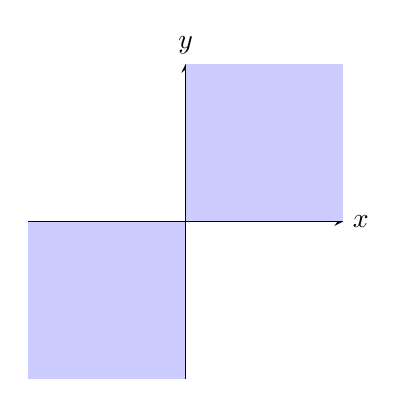
\begin{tikzpicture}[scale=1]
    % Ejes
    \draw[-stealth] (-2,0) -- (2,0) node[right] {\(x\)};
    \draw[-stealth] (0,-2) -- (0,2) node[above] {\(y\)};

    % Región x>0, y>0 (primer cuadrante)
    \fill[blue!20] (0.01,0.01) rectangle (2,2);

    % Región x<0, y<0 (tercer cuadrante)
    \fill[blue!20] (-2,-2) rectangle (-0.01,-0.01);
\end{tikzpicture}
    \caption{En azúl el conjunto $A^\circ$, que junto con los ejes forma $A$.}
\end{figure}
Una forma de probar que $A$ es conexo es mediante una de las últimas proposiciones vistas en teoría sobre la conexión:
\begin{equation*}
    A \text{\ es conexo} \Longleftrightarrow \forall x,y\in A~\exists C\subset A \text{\ conexo con\ } x,y\in C
\end{equation*}
Para ello, la estrategia será demostrar que dado cualquier punto de $A$, el segmento que une dicho punto con el origen se queda contenido en $A$, con lo que podemos unir dos puntos cualesquiera de $A$ pasando por el origen. De esta forma, el conjunto no es convexo, pero resulta que fijado un punto, la propiedad de contener un segmento de cualquier otro extremo sí que se cumple. Este tipo de conjuntos reciben el nombre de \textit{conjuntos estrellados}.\\

\noindent
Comenzando con la demostración, sea $(x,y)\in A$, probemos que:
\begin{equation*}
    Seg(x,y) = \{t(x,y) : t\in [0,1]\} \subset A
\end{equation*}
Para ello, si $(u,v)\in Seg(x,y)$, entonces $\exists t\in [0,1]$ de forma que:
\begin{equation*}
    (u,v) = t(x,y) = (tx,ty)
\end{equation*}
Por lo que:
\begin{equation*}
    uv = t^2xy \geq 0 \Longrightarrow (u,v) \in A
\end{equation*}
Por ser $t^2 \geq 0 $ y $xy \geq 0$. Además, $Seg(x,y)$ es conexo para todo $(x,y)\in A$, ya que dado $(x,y)\in A$ podemos definir $f:[0,1]\to \mathbb{R}^2$ dada por:
\begin{equation*}
    f(t) = t(x,y) \qquad \forall t\in [0,1]
\end{equation*}
Con lo que:
\begin{equation*}
    f([0,1]) = \{t(x,y) : t\in [0,1]\} = Seg(x,y)
\end{equation*}
Como $f$ es continua y $[0,1]$ es conexo por ser un intervalo de $\mathbb{R}$, tenemos que $Seg(x,y)$ es conexo $\forall (x,y)\in A$.\\

\noindent
Ahora, si $(x,y),(u,v)\in A$, podemos considerar $Seg(x,y),Seg(u,v)\subset A$, de forma que:
\begin{itemize}
    \item $(x,y),(0,0)\in Seg(x,y)$.
    \item $(u,v),(0,0)\in Seg(u,v)$.
\end{itemize}
De esta forma, tenemos que $(0,0)\in Seg(x,y)\cap Seg(u,v)\neq \emptyset $, y como ambos son conexos, resulta que $Seg(x,y)\cup Seg(u,v)$ es un conjunto conexo que contiene a $(x,y)$ y a $(u,v)$; por lo que $A$ es conexo.\\

\noindent
Para probar que $A^\circ$ no es conexo, empecemos probando que\footnote{Todavía no lo sabemos, solo tenemos una intuición.}:
\begin{equation*}
    A^\circ = \{(x,y)\in \mathbb{R}^2 : xy > 0\}
\end{equation*}
\begin{description}
    \item [$\supseteq)$] Sea $\varphi:\mathbb{R}^2 \to \mathbb{R}$ dada por:
        \begin{equation*}
            \varphi(x,y) = xy \qquad \forall (x,y)\in \mathbb{R}^2
        \end{equation*}
        Tenemos que:
        \begin{equation*}
            \varphi^{-1}(\mathbb{R}^+) = \{(x,y)\in \mathbb{R}^2 : xy = \varphi(x,y) > 0\}
        \end{equation*}
        Por lo que este conjunto es un abierto contenido en $A$, luego está dentro de $A^\circ$.
    \item [$\subseteq)$] Sea $U\subset A$ un conjunto abierto, si suponemos que $\exists (x,y)\in U$ con $xy = 0$, entonces $x = 0$ o $y = 0$; en cualquiera de estos dos casos, tendremos que $B((x,y),\delta) \not\subset U$ $\forall \delta>0$, por lo que $U$ no es abierto, contradicción que viene de suponer que hay un punto en $U$ que verifica $xy = 0$, por lo que $xy > 0$ para todo $(x,y)\in U$, es decir, $U\subset \{(x,y)\in \mathbb{R}^2 : xy > 0\}$.
\end{description}
Una vez conocida la forma de $A^\circ$, si tomamos:
\begin{equation*}
    U = \{(x,y)\in \mathbb{R}^2 : x,y < 0\}, \qquad V = \{(x,y)\in \mathbb{R}^2 : x,y>0\}
\end{equation*}
Es claro que:
\begin{equation*}
    U\cup V = A^\circ, \qquad U\cap V = \emptyset, \qquad U, V \neq \emptyset 
\end{equation*}
Finalmente, como $\mathbb{R}^-$ y $\mathbb{R}^+$ son abiertos en $\mathbb{R}$ y:
\begin{equation*}
    U = \mathbb{R}^- \times \mathbb{R}^-, \qquad V = \mathbb{R}^+ \times \mathbb{R}^+
\end{equation*}
Concluimos que $U,V$ son abiertos en $\mathbb{R}^2$. En definitiva, $A^\circ$ no es conexo.
\end{ejercicio}

\begin{ejercicio}\label{ej:rel4_11}
Sea \( X \) un espacio normado. Probar que para cualesquiera \( x, y \in X \setminus \{0\} \) se tiene
\[
    \left\| \frac{x}{\|x\|} - \frac{y}{\|y\|} \right\| \leq \frac{2\left\| x - y \right\|}{\|x\|}
\]
Deducir que la función \( \varphi : X \setminus \{0\} \rightarrow X \), dada por \( \varphi(x) = \dfrac{x}{\|x\|} \) para todo \( x \in X \setminus \{0\} \), es continua.\\

\noindent
En primer lugar:
\begin{align*}
    \left\|\dfrac{x}{\|x\|}-\dfrac{y}{\|y\|}\right\| &= \left\|\dfrac{x}{\|x\|} - \dfrac{y}{\|x\|} + \dfrac{y}{\|x\|}-\dfrac{y}{\|y\|}\right\| \leq \left\|\dfrac{x}{\|x\|} - \dfrac{y}{\|x\|}\right\| +\left\| \dfrac{y}{\|x\|}-\dfrac{y}{\|y\|}\right\| \\
                                                     &= \dfrac{1}{\|x\|} \|x-y\| + \left\| y\left(\dfrac{1}{\|x\|}-\dfrac{1}{\|y\|}\right)\right\| = \dfrac{1}{\|x\|} \|x-y\| +\left| \dfrac{1}{\|x\|}-\dfrac{1}{\|y\|}\right| \|y\| \\
                                                     & \forall x,y\in X\setminus \{0\}
\end{align*}
Ahora:
\begin{equation*}
    \left| \dfrac{1}{\|x\|}-\dfrac{1}{\|y\|}\right| \|y\|  = \dfrac{|\|y\|-\|x\||}{\|x\|\|y\|} \|y\|  \leq \dfrac{\|x-y\|}{\|x\|} \qquad \forall x,y\in X\setminus \{0\}
\end{equation*}
Por lo que:
\begin{equation*}
    \left\| \frac{x}{\|x\|} - \frac{y}{\|y\|} \right\| \leq \frac{\left\| x - y \right\|}{\|x\|} + \frac{\left\| x - y \right\|}{\|x\|} = \frac{2\left\| x - y \right\|}{\|x\|} \qquad  \forall x,y\in X\setminus \{0\}
\end{equation*}
Si ahora consideramos la función $\varphi:X\setminus \{0\}\to X$ dada por:
\begin{equation*}
    \varphi(x) = \dfrac{x}{\|x\|} \qquad \forall x\in X\setminus \{0\}
\end{equation*}
Fijado $x\in X$, dado $\varepsilon>0$, si $y\in X\setminus\{0\}$ con:
\begin{equation*}
    \|y-x\| = \|x-y\| < \dfrac{\|x\|\varepsilon}{2} = \delta
\end{equation*}
Entonces:
\begin{equation*}
    \|\varphi(y) - \varphi(x)\| = \left\| \frac{x}{\|x\|} - \frac{y}{\|y\|} \right\|\leq \frac{2\left\| x - y \right\|}{\|x\|} < \frac{2\|x\|\varepsilon}{2\|x\|} =  \varepsilon
\end{equation*}
Por lo que $\varphi$ es continua en $x$, $\forall x\in E$.
\end{ejercicio}

\begin{ejercicio}
Probar que, si \( X \) es un espacio normado de dimensión mayor que 1, el conjunto \( X \setminus \{0\} \) es conexo. Deducir que la \textit{esfera unidad} dada por la ecuación \( S(0,1) = \{ x \in X : \|x\| = 1 \} \) es un conjunto conexo.\\

\noindent
Usaremos la misma proposición que usamos en el Ejercicio~\ref{ej:rel4_10}. Para ello, sean $x,y\in X\setminus \{0\}$:
\begin{itemize}
    \item Si $x$ e $y$ son linealmente independientes, entonces la recta que pasa por dichos dos puntos:
        \begin{equation*}
            R(x,y) = \{tx + (1-t)y : t\in \mathbb{R}\}
        \end{equation*}
        no contiene al cero, ya que si $0\in R(x,y)$, entonces $\exists t\in \mathbb{R}^\ast$ (ya que si $t=0$, entonces $0=y\in X\setminus \{0\}$) de forma que:
        \begin{equation*}
            tx + (1-t)y = 0 \Longrightarrow x = \dfrac{t-1}{t}y
        \end{equation*}
        Por lo que $x$ e $y$ son linealmente dependientes, contradicción. De esta forma, tenemos que $R(x,y)$ es un conjunto convexo, luego conexo, contenido en $X\setminus \{0\}$ que contiene a $x$ y a $y$; por lo que podemos ``conectar'' cualesquiera dos puntos linealmente independientes en $X\setminus \{0\}$.
        \begin{figure}[H]
            \centering
            \begin{tikzpicture}[scale=2]
              % Ejes coordenados
              \draw[-stealth] (-0.5,0) -- (1.5,0) node[right] {};
              \draw[-stealth] (0,-1.5) -- (0,0.5) node[above] {};
              
              % Puntos
              \filldraw[blue] (1,0) circle (1pt) node[below right] {$x$};
              \filldraw[blue] (0,-1) circle (1pt) node[below right] {$y$};
              
              % Recta que pasa por ambos puntos (prolongación)
              \draw[red, thick, domain=-0.5:1.5] plot (\x, {-1 + \x});
              
            \end{tikzpicture}
            \caption{Cómo conectar dos puntos linealmente independientes.}
        \end{figure}
    \item Si $x$ e $y$ son linealmente dependientes, entonces $\exists \lm \in \mathbb{R}$ de forma que $y = \lm x$. Distinguimos casos:
        \begin{itemize}
            \item Si $\lm = 0$, entonces $y = 0$, pero $y \in X\setminus \{0\}$, por lo que este caso es imposible.
            \item Si $\lm > 0$, podemos repetir el razonamiento anterior tomando:
                \begin{equation*}
                    Seg(x,y) = \{tx + (1-t)y : t \in [0,1]\}
                \end{equation*}
                que no contiene al cero, ya que si $0\in Seg(x,y)$, entonces $\exists t\in [0,1]$ de forma que:
                \begin{equation*}
                    0 = tx + (1-t)y \Longrightarrow  tx = (t-1)\lm x \Longrightarrow t = (t-1)\lm \Longrightarrow \lm = \dfrac{t}{t-1} < 0
                \end{equation*}
                contradicción, por lo que $0 \notin Seg(x,y)$, luego $Seg(x,y) \subset X\setminus \{0\}$, con $x,y\in Seg(x,y)$ y dicho conjunto es convexo, luego conexo.
        \begin{figure}[H]
            \centering
            \begin{tikzpicture}[scale=2]
              % Ejes coordenados
              \draw[-stealth] (-0.5,0) -- (3.5,0) node[right] {};
              \draw[-stealth] (0,-0.5) -- (0,0.5) node[above] {};
              
              % Puntos
              \filldraw[blue] (2,0) circle (1pt) node[below right] {$x$};
              \filldraw[blue] (1,0) circle (1pt) node[below right] {$y$};
              
              % Recta que pasa por ambos puntos (prolongación)
              \draw[red, thick, domain=1:2] plot (\x, {0});
              
            \end{tikzpicture}
            \caption{Cómo conectar dos puntos linealmente dependientes positivamente.}
        \end{figure}
    \item Si $\lm < 0$, como $dim X > 1$, existe $z\in X\setminus \{0\}$ linealmente independiente con $x$, luego también es linealmente independiente con $y$. Usando el primer caso, tenemos que $R(x,z), R(y,z)$ son dos conjuntos conexos con:
        \begin{itemize}
            \item $x,z\in R(x,z)$.
            \item $y,z\in R(y,z)$.
        \end{itemize}
        Por lo que $R(x,z)\cap R(y,z)\neq \emptyset $, con lo que $R(x,z)\cup R(y,z)$ es un conjunto conexo con $x,y\in R(x,z)\cup R(y,z)$.
        \begin{figure}[H]
            \centering
            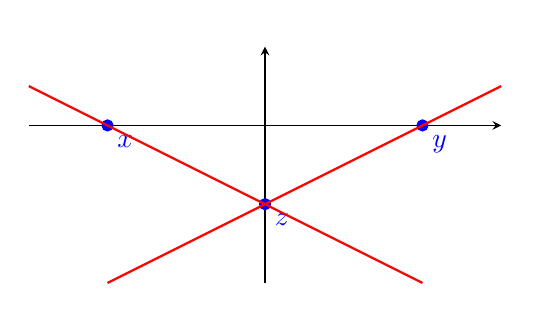
\begin{tikzpicture}[scale=2]
              % Ejes coordenados
              \draw[-stealth] (-1.5,0) -- (1.5,0) node[right] {};
              \draw[-stealth] (0,-1) -- (0,0.5) node[above] {};
              
              % Puntos
              \filldraw[blue] (-1,0) circle (1pt) node[below right] {$x$};
              \filldraw[blue] (1,0) circle (1pt) node[below right] {$y$};
              \filldraw[blue] (0,-0.5) circle (1pt) node[below right] {$z$};
              
              % Recta que pasa por ambos puntos (prolongación)
              \draw[red, thick, domain=-1:1.5] plot (\x, {1/2*\x - 0.5});
              \draw[red, thick, domain=-1.5:1] plot (\x, {-1/2*\x - 0.5});
              
            \end{tikzpicture}
            \caption{Cómo conectar dos puntos linealmente dependientes negativamente.}
        \end{figure}
        \end{itemize}
        En definitiva, $X\setminus \{0\}$ es conexo. Sea ahora:
        \begin{equation*}
            S(0,1) = \{x\in X : \|x\| = 1\}
        \end{equation*}
        Si definimos $\varphi:X\setminus \{0\} \to X$ dada por:
        \begin{equation*}
            \varphi(x) = \dfrac{x}{\|x\|} \qquad \forall x\in X\setminus\{0\}
        \end{equation*}
        Tenemos por el Ejercicio~\ref{ej:rel4_11} que $\varphi$ es continua, y como acabamos de ver que $X\setminus\{0\}$ es conexo, tenemos que $\varphi(X\setminus\{0\})$ es también un conexo. Veamos finalmente que $\varphi(X\setminus\{0\}) = S(0,1)$:
        \begin{description}
            \item [$\subseteq)$] Sea $x\in X\setminus\{0\}$, entonces:
                \begin{equation*}
                    \|\varphi(x)\| = \left\|\dfrac{x}{\|x\|}\right\| = \dfrac{1}{\|x\|} \|x\| = 1
                \end{equation*}
                Luego $\varphi(x) \in S(0,1)$, para todo $x\in X\setminus\{0\}$.
            \item [$\supseteq)$] Sea $x\in S(0,1)\subset X\setminus\{0\}$, entonces:
                \begin{equation*}
                    \varphi(x) = \dfrac{x}{\|x\|} = x
                \end{equation*}
                Luego $x\in \varphi(X\setminus \{0\})$.
        \end{description}
\end{itemize}
\end{ejercicio}
